\documentclass[journal]{IEEEtran}

\usepackage{cite}
\usepackage[pdftex]{graphicx}
\graphicspath{{figures/}}
\DeclareGraphicsExtensions{.pdf,.jpeg,.jpg,.png}
\usepackage[cmex10]{amsmath}
\usepackage{algorithmic}
\usepackage[caption=false,font=normalsize,labelfont=sf,textfont=sf]{subfig}
\usepackage{fixltx2e}
\usepackage{stfloats}


% correct bad hyphenation here
\hyphenation{op-tical net-works semi-conduc-tor}

% Load basic packages
\usepackage{balance}  % to better equalize the last page
\usepackage{graphics} % for EPS, load graphicx instead
\usepackage{times}    % comment if you want LaTeX's default font
\usepackage{url}      % llt: nicely formatted URLs
%\usepackage{flushend} % bjoern: attempt to balance last page
\usepackage[]{algorithm2e}
\let\proof\relax
\let\endproof\relax
\usepackage{amsthm}
\newtheorem{theorem}{Theorem}

% llt: Define a global style for URLs, rather that the default one
\makeatletter
\def\url@leostyle{%
  \@ifundefined{selectfont}{\def\UrlFont{\sf}}{\def\UrlFont{\small\bf\ttfamily}}}
\makeatother
\urlstyle{leo}

\usepackage[pdftex]{hyperref}
\hypersetup{
pdftitle={SIGCHI Conference Proceedings Format},
pdfauthor={LaTeX},
pdfkeywords={SIGCHI, proceedings, archival format},
bookmarksnumbered,
pdfstartview={FitH},
colorlinks,
citecolor=black,
filecolor=black,
linkcolor=black,
urlcolor=black,
breaklinks=true,
}

\begin{document}

%!TEX root = brainreader.tex

%use these commands while writing
\newcommand {\valkyrie}[1]{{\bf{VS: #1}\normalfont}}
\newcommand {\natalia}[1]{{\bf{NB: #1}\normalfont}}
%\newcommand {\changes}[1]{{\color{changes}{#1}\normalfont}}
\newcommand {\changes}[1]{{#1}}

%uncomment these for final submit
%\renewcommand {\valkyrie}[1]{}
%\renewcommand {\natalia}[1]{}

\newcommand{\noopsort}[2]{#2}

\newcommand {\bt}[1]{\textbf{#1} \normalfont}
\newcommand{\squishlist}{
 \begin{list}{$\bullet$}
  { \setlength{\itemsep}{0pt}
     \setlength{\parsep}{3pt}
     \setlength{\topsep}{3pt}
     \setlength{\partopsep}{0pt}
     \setlength{\leftmargin}{1.5em}
     \setlength{\labelwidth}{1em}
     \setlength{\labelsep}{0.5em} } }
\newcommand{\squishend}{
  \end{list}  }

\newenvironment{packed_enum}{
\begin{enumerate}
  \setlength{\itemsep}{1pt}
  \setlength{\parskip}{0pt}
  \setlength{\parsep}{0pt}
}{\end{enumerate}}

\newenvironment{packed_desc}{
\begin{description}
  \setlength{\itemsep}{1pt}
  \setlength{\parskip}{0pt}
  \setlength{\parsep}{0pt}
}{\end{description}}

%
% paper title
% Titles are generally capitalized except for words such as a, an, and, as,
% at, but, by, for, in, nor, of, on, or, the, to and up, which are usually
% not capitalized unless they are the first or last word of the title.
% Linebreaks \\ can be used within to get better formatting as desired.
% Do not put math or special symbols in the title.
\title{BrainReader: Effective Visualization\\of fMRI-based Movie Reconstruction}
%
%
% author names and IEEE memberships
% note positions of commas and nonbreaking spaces ( ~ ) LaTeX will not break
% a structure at a ~ so this keeps an author's name from being broken across
% two lines.
% use \thanks{} to gain access to the first footnote area
% a separate \thanks must be used for each paragraph as LaTeX2e's \thanks
% was not built to handle multiple paragraphs
%

\author{Natalia Bilenko, Valkyrie Savage% <-this % stops a space
\thanks{Natalia and Valkyrie are joint first-authors on this work.  They can be reached via email at \emph{nbilenko@berkeley.edu} and \emph{valkyrie@eecs.berkeley.edu}.}% <-this % stops a space
\thanks{Manuscript submitted December 18th, 2014.}}



% The paper headers
\markboth{Computational Photography Final Project, CS 294-84, December 2014}%
{Bilenko and Savage: BrainReader}



% If you want to put a publisher's ID mark on the page you can do it like
% this:
%\IEEEpubid{0000--0000/00\$00.00~\copyright~2014 IEEE}
% Remember, if you use this you must call \IEEEpubidadjcol in the second
% column for its text to clear the IEEEpubid mark.



% use for special paper notices
%\IEEEspecialpapernotice{(Invited Paper)}




% make the title area
\maketitle

% As a general rule, do not put math, special symbols or citations
% in the abstract or keywords.
\begin{abstract}
Previous work in decoding visual experiences based on fMRI activity has been successful in reconstructing images and movies that participants viewed inside an MRI scanner. Reconstruction is done by fitting a forward model that predicts fMRI activity across the brain in response to a set of movies. The model represents brain activity as a linearized function of visual information features that capture the structure of the movies (spatiotemporal Gabor wavelet filters). The forward model is then inverted and used to decode what the subject saw based on their brain responses to a testing set of movies. Decoding is performed by fitting a maximum a posteriori function to a large library of previously unseen movie clips. The top 100 decoded movie clips are then averaged or stitched together to produce a visualization of the decoding. Though the decoding is quite precise when measured quantitatively, these visualizations do not fully reflect its accuracy. We make the visualization more coherent by combining the decoded clips in several improved ways. First, we demonstrate the change in quality gained using weighted averaging.  Then, we use HOG features to select a subset clips similar to the ground truth clip and SIFT flow to find an optimal path in time. Third, we use appearance morphing to visually align the path-arranged clips. Finally, we share the decoded movies resulting from the same stimuli across different participants in the experiment.
\end{abstract}

% Note that keywords are not normally used for peerreview papers.
\begin{IEEEkeywords}
fMRI, decoding, visualization, computational videography.
\end{IEEEkeywords}


\IEEEpeerreviewmaketitle

%!TEX root = brainreader.tex

\section{Introduction}
\IEEEPARstart{F}{unctional} magnetic resonance imaging, or fMRI, is a technology used in neuroscientific research for recording brain activity. It can be used for a technique called ``brain decoding'', which refers to identifying sensory stimuli or brain states that an individual is experiencing, based on their brain activity. Researchers have been able to use fMRI data to decode visual stimuli in several fMRI studies (\cite{Kamitani}; \cite{Naselaris}; \cite{Nishimoto}).

The most complex reconstruction of visual information to date was done by Nishimoto and colleagues in the Gallant lab at UC Berkeley. The researchers built a forward model predicting fMRI signals in the visual cortex from the structural content in the movies seen by the subject. The structural content was captured by processing the movies with spatiotemporal motion energy filters. These filters represent spatial frequency, temporal frequency, and orientation features at different scales and locations on the screen. 

Ridge regression was used to fit a predictive model between the motion energy parameterization of the movies and the fMRI responses at each recording site (voxel) in the brain. A Bayesian approach was then used to build the inverse model. The posterior probability of the movie decoded from brain activity was estimated by combining a likelihood function given by the forward model and a natural movie prior. In the absence of an explicit distribution of natural images, the natural prior was simulated by sampling 18,000,000 seconds of videos from YouTube.

The model was successful, and using the likelihood of brain activity to identify each timepoint in a held-out stimulus set produced the correct result 95\% of the time. To visualize the result of the direct decoding using the natural movie prior, a set of 100 clips with the highest log likelihood according to the model was selected and averaged. The resulting video can be viewed here (http://www.youtube.com/watch?v=nsjDnYxJ0bo). While the decoding results are quite accurate as seen from the identification, the video appears fuzzy and is misleading about the precision of the decoding. Using computational techniques, we can improve the quality of these output videos (Figure \ref{fig:avg})


\begin{figure}[t]
\centering
    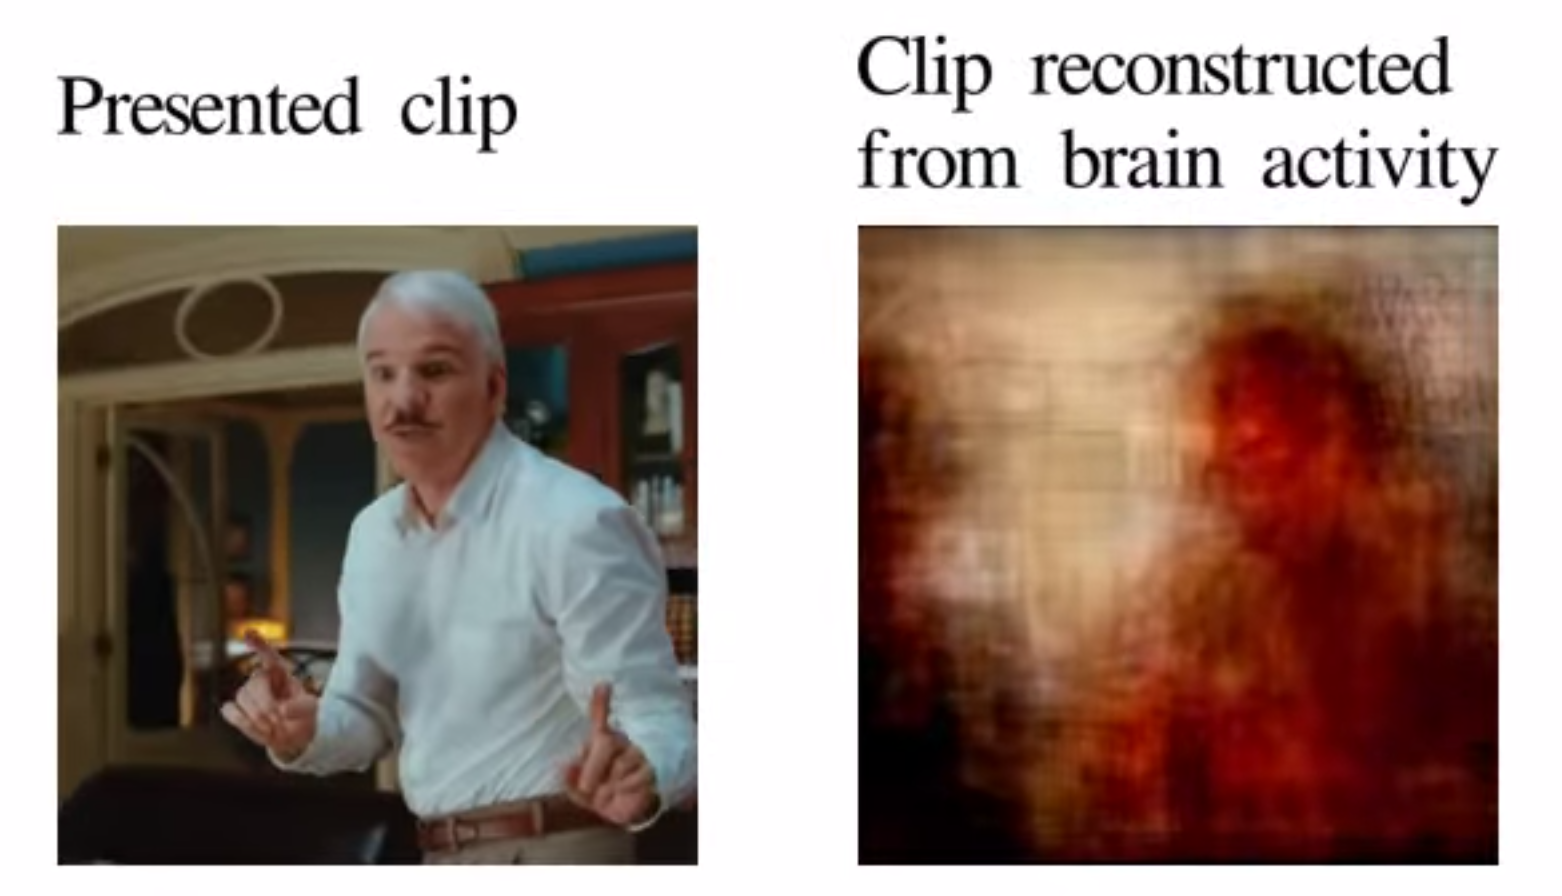
\includegraphics[width=1.0\columnwidth]{figures/average.png}
\caption{a) The first generation of visualization for BrainReader clips: the top 100 guesses are simply averaged and overlaid to create an output image at each frame.  This belies the accuracy of the technique, which is quite high. b) Our improved visualization \valkyrie{obviously need image here.}.}
\label{fig:avg}
\end{figure}


Instead of a simple averaging process for turning guesses into an output video, we used several more sophisticated approaches.  First, we simply performed weighted averaging, using relative log likelihood scores of the clips as our weights.  This already constituted an improvement over na\"{i}ve weighting (Figure \ref{fig:weighted}).

\begin{figure}[t]
\centering
    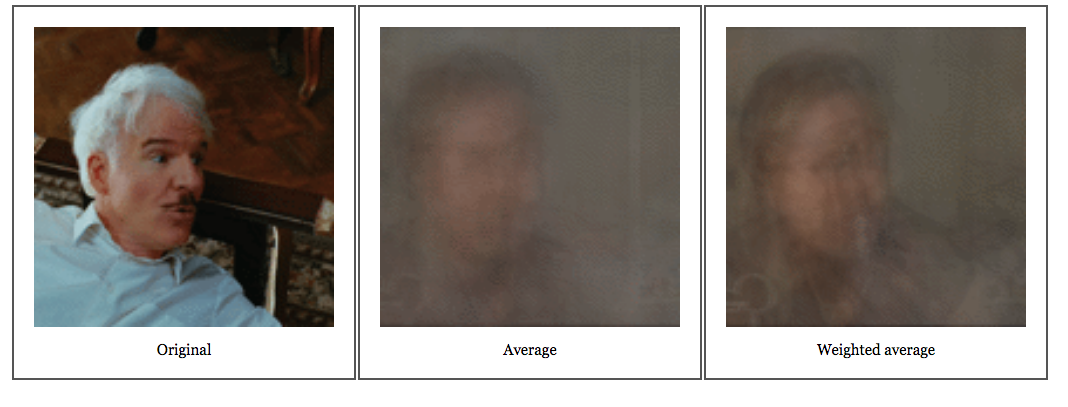
\includegraphics[width=1.0\columnwidth]{figures/orig-avg-weighted.png}
\caption{Using a weighted average improves over the na\"{i}ve average.  Left: original clip presented.  Center: na\"{i}ve average.  Right: weighted average.}
\label{fig:weighted}
\end{figure}


After using weighted averaging, we turned to even more sophisticated techniques: HOG feature alignment and SIFT flow.  These give us additional information on the edges makeup and semantic scene composition of both the original clip and the top 100 guesses as predicted by the original fMRI-based system.  We perform three steps to create our visualization from these ranked guesses: pruning, consistency-assurance, and visual morphing.

%!TEX root = brainreader.tex

\section{Methods}

Our processing pipeline takes as input two pieces of data for each second:

\begin{itemize}
\item The top 100 guesses (based on fMRI data) - each guess has 15 frames
\item The log-likelihood (LLH) of each guess
\end{itemize}

We experimented with a variety of options for the 5 core steps of \emph{Weeding}, \emph{Forced Alignment}, \emph{Flow Calculation}, \emph{Pathfinding}, and \emph{Visualization} (see Figure \ref{fig:system}).

\begin{figure}
\centering
    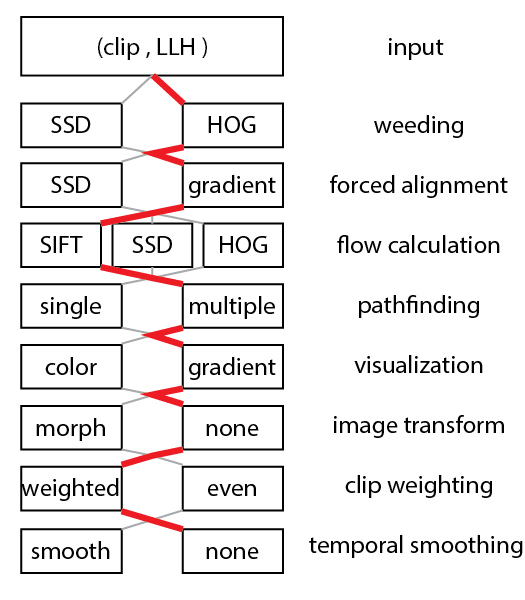
\includegraphics[width=1.0\columnwidth]{figures/system.png}
\caption{We experimented with a variety of options for the core steps of Preprocessing, Forced Alignment, Flow Calculation, Pathfinding, and Visualization (including method, image transformation, clip weighting, and temporal smoothing).  Highlighted in red is the path that was chosen.}
\label{fig:system}
\end{figure}

There are a few processes that we used for several steps in our pipeline, described here for later reference:

\emph{SSD} - Sum of Squared Differences (SSD) is a single number that represents a ``match'' score between two images.  It takes into account differences across the images' respective color channels, squaring and summing those differences to create one number indicating overall different-ness.

\emph{HOG} - Histogram of Oriented Gradients (HOG) descriptors focus on an image's edge data.  The descriptor has a variety of bins representing orientations and locations: images with similar HOG descriptors have similar edge orientations in similar spatial locations \cite{HOG}.

\emph{Gradient} - An image's gradient magnitude is equal to the square root of the sum of squares of the x-gradient and y-graident and represents change in the image rather than absolute values.  Large changes in the image typically correspond to edges.

\subsection{Weeding}
While the 100 clips are already chosen to correspond to the fMRI data by the log-likelihood values of the model, in order to make an effective visualization we first discard clips that have very jarring transitions between timepoints. By minimizing the change in the content of the first frame of each clip and the last frame of the previous clip, we smooth the set of clips to one with smoother transitions.

We attempted two processes for this: \emph{SSD} and \emph{HOG}.  Intuitively, SSD should be better for preserving color across clips, since it takes color into account, while HOG should be better at preserving the edge content from one clip to another.  Therefore, we would expect that HOG-weeded guess clips would have better shape consistency.  This appears to be true to some degree (see Figure \ref{fig:weeding}): therefore we select HOG as our weeding tool of choice (in spite of SSD's obvious superiority in time efficiency).

\begin{figure}
\centering
    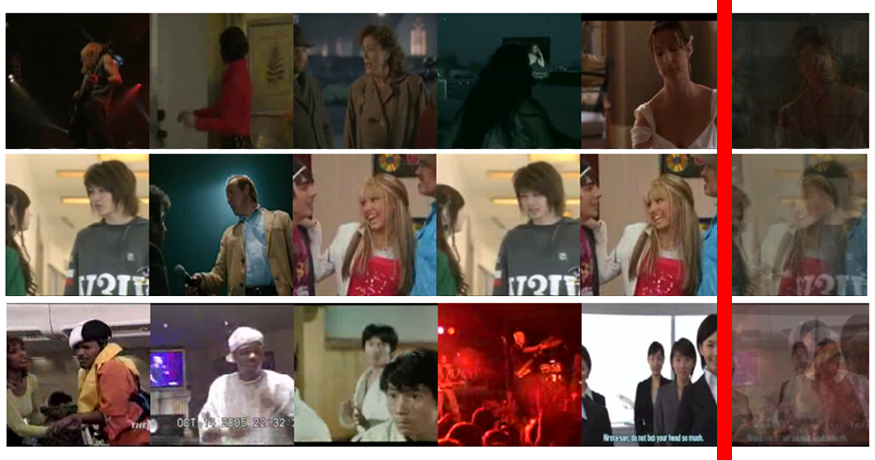
\includegraphics[width=0.95\columnwidth]{figures/preproc.png}
\caption{The top 5 guesses for one frame weeded based on SSD (top), HOG (middle), and LLH (bottom); and the sum of all five images (right).}
\label{fig:weeding}
\end{figure}

\subsection{Forced Alignment}
We forcibly align our guesses to each other: this makes the final visualization more pleasing, in addition to making flow calculations (discussed next) more meaningful. This precision of decoded alignment cannot be exact with fMRI data, and thus this alignment is justified. Although some neurons, particularly in early visual areas, are tuned precisely to very small portions of the visual field, fMRI voxels average over hundreds of thousands of neurons, and such fine tuning is lost. Nonetheless, voxels are spatially tuned, well enough to recover retinotopic organization of the visual areas, but this tuning is at less than pixel accuracy. Thus we can improve our visualization by alignment at a pixel level.

The two forced alignment metrics we tested were \emph{SSD} and \emph{gradient}.

SSD-based alignment forcing encourages alignment of colors, while gradient-based alignment encourages alignment of edges.  Depending on the final visualization configuration, either may be desirable: if the visualization is going to be compiled in the color domain, color-based alignment may be best.  However, alignment in the gradient domain is more suited to visualization in the gradient domain (see Figure \ref{fig:align}).

\begin{figure}
\centering
    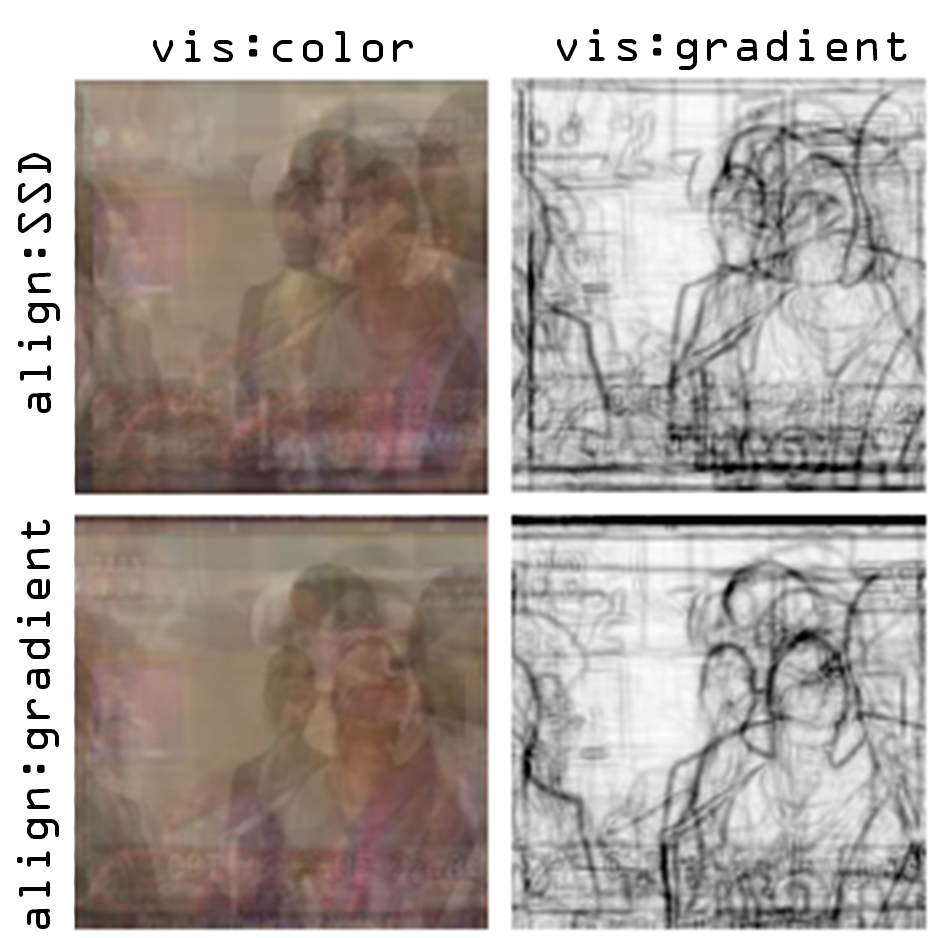
\includegraphics[width=1.0\columnwidth]{figures/align.png}
\caption{SSD-based alignment and gradient-based alignment lend themselves to different visualization techniques.  Here we show all possibilities of alignment technique x visualization technique: note that the lines match up best in the gradient domain when alignment is done there, and colors match up best when SSD is the alignment technique.}
\label{fig:align}
\end{figure}

For our final videos, we selected to use gradient-based alignment: visualizing our output in the gradient domain is more ``true'' to the fMRI data, which only accounts for shape and ignores color, and gradient-based alignment lends itself to gradient-based visualization.

\subsection{Flow Calculation}
We elected to reduce the number of clips shown in the final visualization from 100 to a much smaller number, which allows us some additional flexibility in stringing the clips together.  Instead of needing to create transitions from every clip from one time step into every clip from the next time step, we are able to take one or a few clips from the 100 best guesses and create a smooth path through those clips.

But what makes a ``smooth'' path?  Ideally, a smooth path is one where the last frame of one clip lines up with the first frame of the following clip: various techniques have been tried to determine the ``difference'' between two images.

\emph{SIFT flow} \cite{SIFTflow} finds SIFT keypoints in two images and estimates the ``flow'' of these keypoints between the two images. This type of matching rewards scenes that are semantically, though perhaps not compositionally, similar: e.g., two images of streets would likely have low SIFT flow, while an image with a street at the bottom and an image with a river at the bottom would likely have high SIFT flow.  We found the smoothest paths using SIFT flow. Unfortunately, it is much more computationally expensive than other techniques we tried, but the improvement was much greater.

A second technique for path smoothness is \emph{SSD}.  Used in this part of the pipeline, SSD will ideally minimize jumps in color and composition between adjacent time steps, making clips flow smoothly into each other.

The final flow calculation we implemented was \emph{HOG}-based flow.  This again focuses on edge orientation and location, and lends itself to visualization consistency in the gradient domain.

Both the SSD and HOG techniques are the same as the ones we tried above before aligning the images. Thus, we only use the weeding step for the SIFT flow version of this step.

We compare the various flow calculation techniques tested in Figure \ref{fig:flows} and Figure \ref{fig:comparison}.

\begin{figure}
\centering
    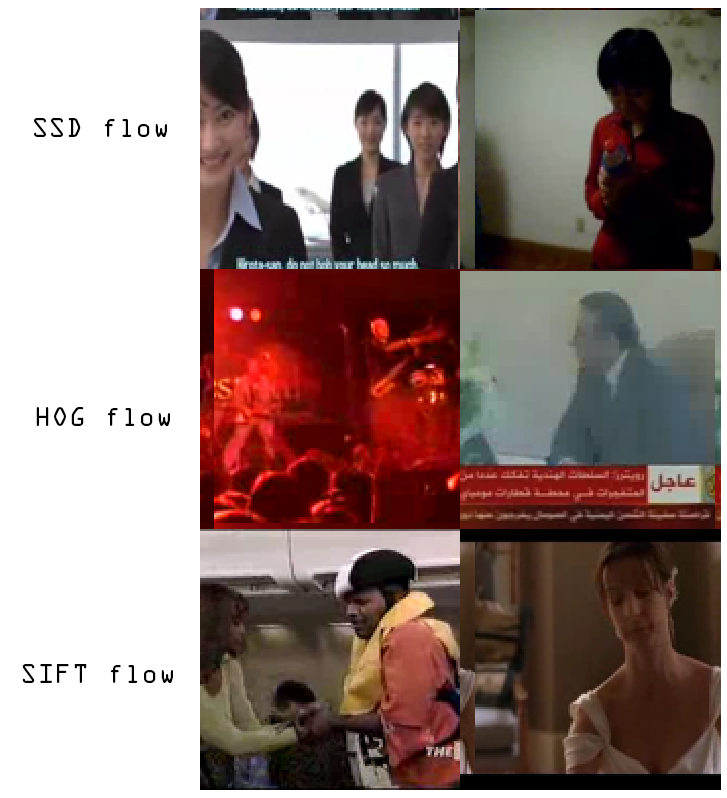
\includegraphics[width=1.0\columnwidth]{figures/lowflowstitled.png}
\caption{Various techniques can be used to calculate the ``difference'' between two images (in our case, the last frame of one clip and the first frame of the following clip).  We implemented SSD (focus on colors), HOG (focus on edges), and SIFT (focus on semantics).}
\label{fig:flows}
\end{figure}

\begin{figure}
\centering
    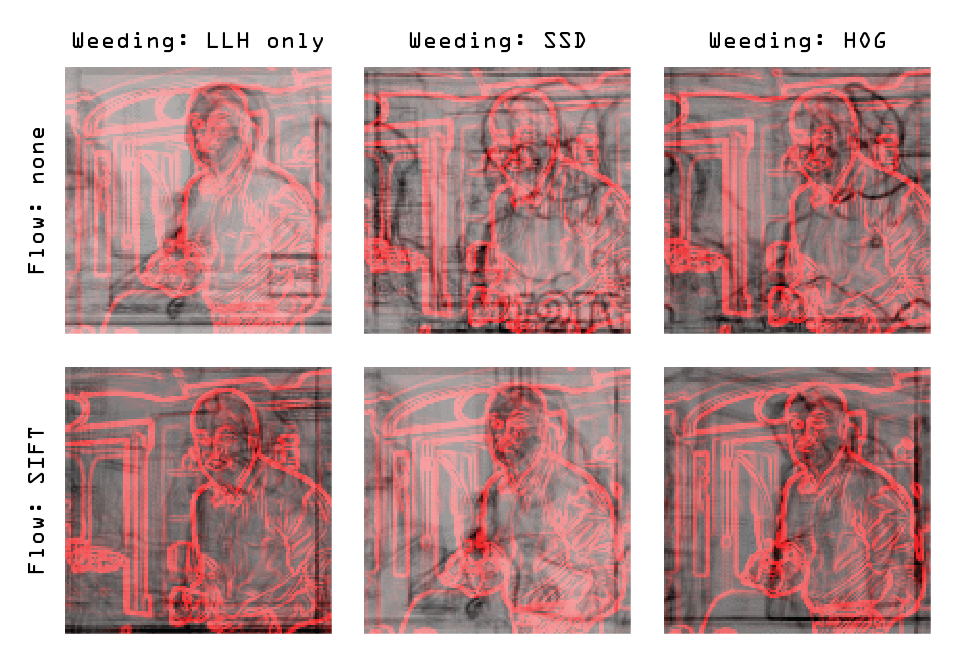
\includegraphics[width=1.0\columnwidth]{figures/methodcomp.png}
\caption{Comparison of techniques to compute the best clip progression. In the top row, the images are weeded out from 100 best clips to 20 best clips using either just the log-likelihood of the fMRI model (LLH), SSD, or HOG features. In the bottom row, SIFT-flow is used to compute the best progression in addition to the weeding. The result is an average of the best 5 clips in the path, visualized as the gradient magnitude with the gradient magnitude of the original clip overlayed in red.}
\label{fig:comparison}
\end{figure}

\subsection{Pathfinding}
To find the optimal path through the clips, the whole set of clips can be seen as a Markov chain. There is a node at each second of the reconstructed movie, and the possible clips for that second representing the states of that node. The flow metrics between each pair of clips constitue the values of the transition matrix between all states. We used dynamic programming to find the optimal path through the transition matrix. First, we found the lowest cumulative cost to get to each consecutive clip in the transition matrix. Then, we backtracked through the transition cost matrix to find the cheapest path for one or several clips. After some testing, we chose a path of five clips, as it produced the most visually appealing results.

\subsection{Visualization}
We visualized the resuling movies in several ways. First, we averaged the clips in the chosen path to obtain one continuous movie. This gave us the most direct comparison to the previous approach of averaging the top 100 clips. Before averaging, we weighted the clips by the relative fMRI model log-likelihood of each clip. See Figure \ref{fig:viz} (a).

\subsubsection{Gradient Domain and Overlay}
The fMRI model is based on spatiotemporal features of the movies, including spatial frequencies and orientations. We wanted to emphasize the decoding of these features by highlighting the edges in the reconstructed movies. To do this, we visualized the reconstructed movies in the gradient domain. The gradient magnitude of all clips was computed. We displayed the inverse magnitude, showing dark edges on a white background. To demonstrate the difference between the reconstructed and original movie, we also computed the gradient of the original movie. We overlayed the original gradient movie in red over the reconstructed gradient movie in black and white. See Figure \ref{fig:viz} (b) and (c).

\begin{figure}
\centering
    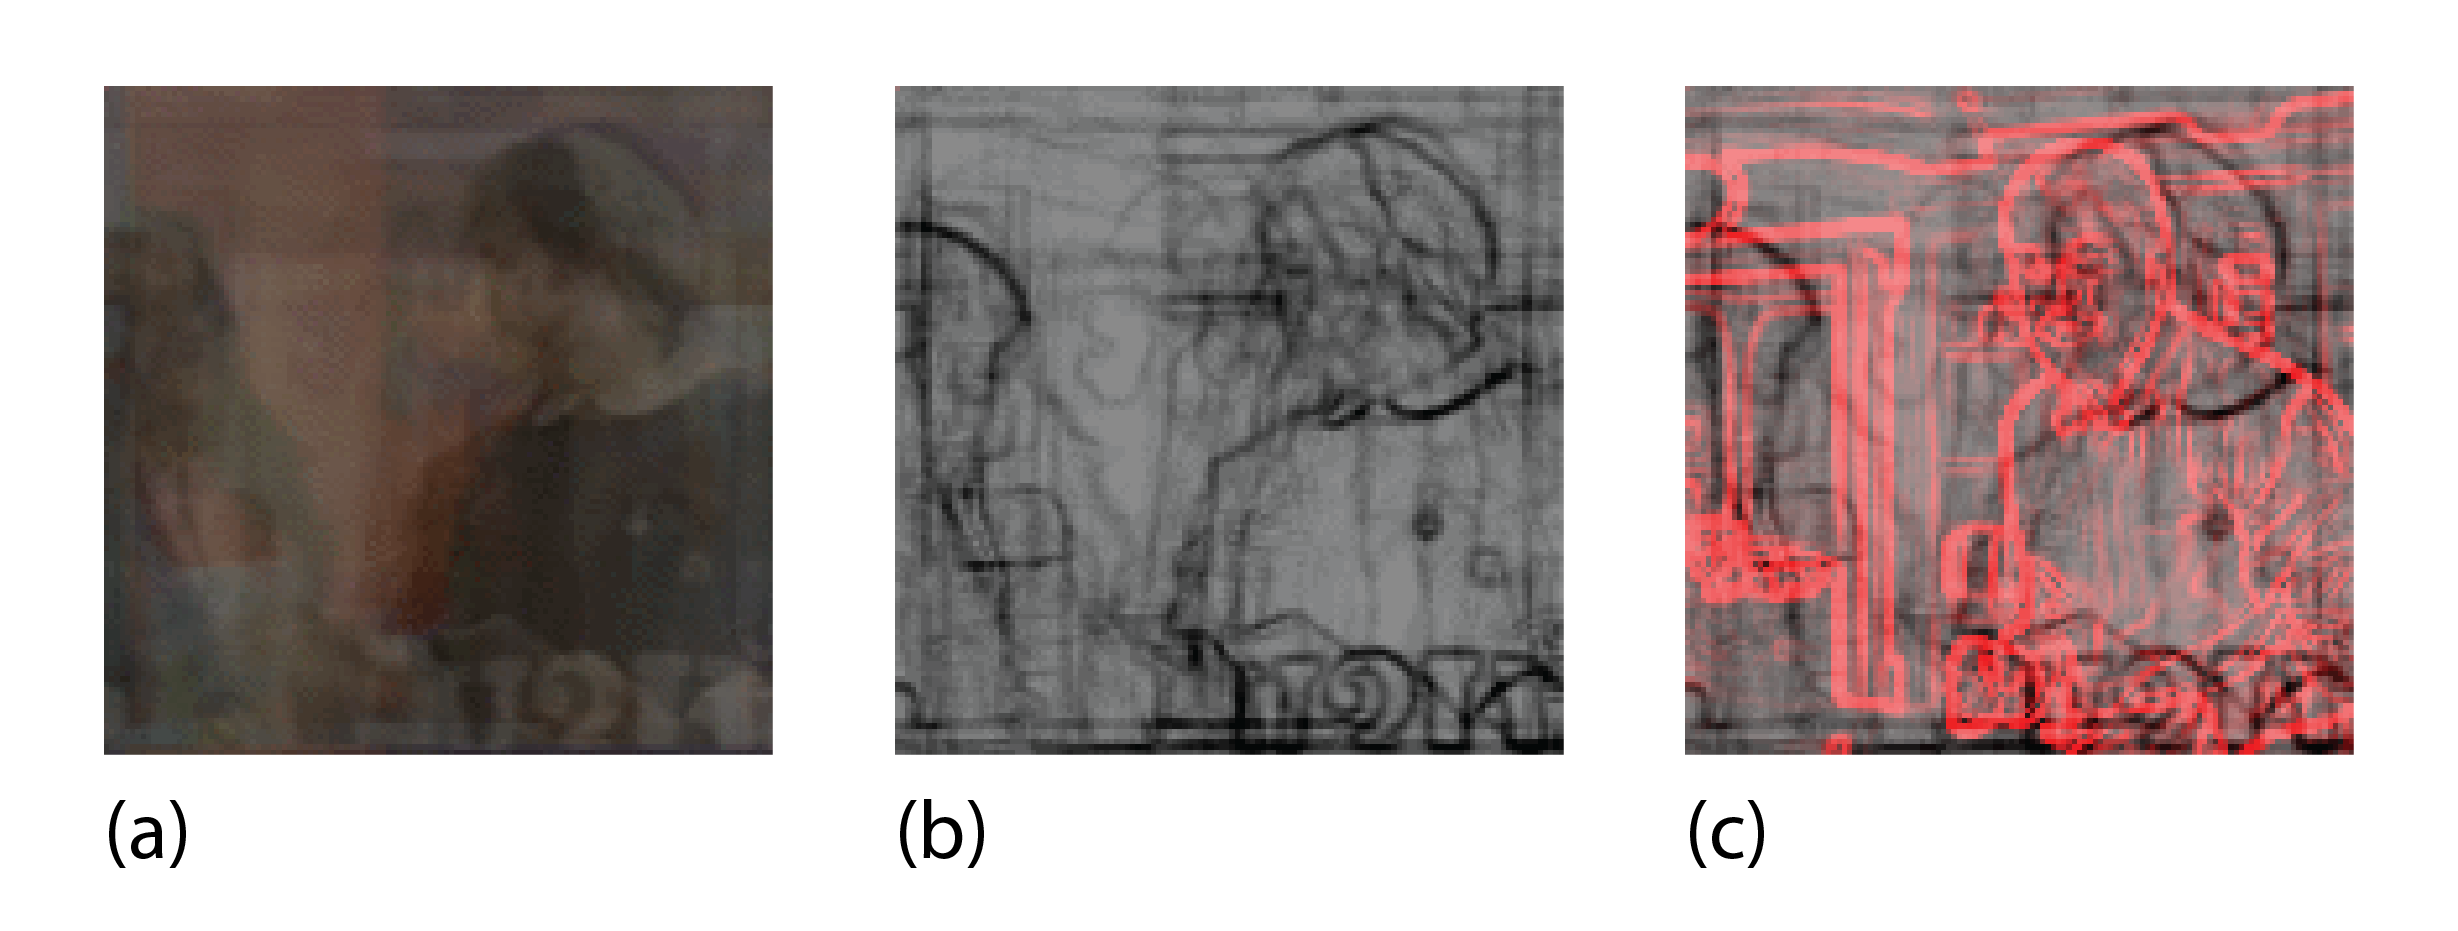
\includegraphics[width=1.0\columnwidth]{figures/vizfig.png}
\caption{Three techniques were used to visualize the results. (a) Top 5 clips found in the smoothest path, weighted by relative log-likelihood and averaged. (b) The same 5 clips, transformed to gradient magnitude before averaging. (c) The same result, withg the radient magnitude of the original clip overlaid in red.}
\label{fig:viz}
\end{figure}

\subsubsection{Smoothing}
To make the appearance of the movie smoother, we averaged the clips temporally with a moving average filter. The averaging was done with each frame weighted by the reciprocal of the window width. We experimented with several sliding window width and chose five frames as the best span.

%!TEX root = brainreader.tex

\section{Related Work}

Our work relates to both basic image processing and video processing.

\subsection{Image Processing}

Most obviously, our work builds off of previous techniques for finding image differences and similarities, like HOG \cite{HOG} and SIFT flow \cite{SIFTflow}.  We use these algorithms wholesale as a component of our pipeline, however our usage of them is slightly different than what was originally proposed: we are neither intentionally detecting humans as in the HOG paper (although we do, incidentally, have a dataset with many humans in it) nor are we trying to align multiple images of the same object as in the SIFT flow paper.

\subsection{Image Search}

Our work is additionally similar to image searching techniques, for example AverageExplorer \cite{averageExplorer}.

%!TEX root = brainreader.tex

\section{Discussion}

As our understanding of the brain becomes more and more precise, this type of visualization will surely get better.  This iteration of the BrainDreamer project lacks information about colors and semantics: addition of both would certainly lead to even more accurate results.

Additionally, some results in our dataset are certainly more convincing than others.  Data for which there are many nearly-precise matchings in the database (for example, of human faces) lead to much nicer visualizations, while more unusual data (for example, nudibranchs and other sea creatures) must have their edges ``re-constituted'' by many near matches overlaid.  This is a limitation of the dataset itself. The database of 18,000,000 seconds of clips is quite diverse, but is still limited. While our alignment and visualization techniques can help, some images in the movie that the people saw cannot be well-matched. Additionally, the decoding is based on fMRI responses in the visual cortex and on a model that captures low-level visual information. Some movie information may be better represented in the brain according to its narrative content and higher-level processing. Thus, some images in the movie may not be well reconstructed due to the limitations of the model.

In future work, it would be beneficial to quantitatively compare our visualization techniques with the decoded fMRI data: for example by measuring distances between presented edges and edges in the final visualization, or by presenting the visualization to subjects to compare the brain's reaction to it with the brain's reaction to the original stimulus.

%!TEX root = brainreader.tex

\section{Conclusion}

We have compared a variety of processing techniques for creating effective visualizations of fMRI data.  Our visualization processing constitutes a huge improvement over previous work, and better indicates the precision of the fMRI technique.




% if have a single appendix:
%\appendix[Proof of the Zonklar Equations]
% or
%\appendix  % for no appendix heading
% do not use \section anymore after \appendix, only \section*
% is possibly needed

% use appendices with more than one appendix
% then use \section to start each appendix
% you must declare a \section before using any
% \subsection or using \label (\appendices by itself
% starts a section numbered zero.)
%


%\appendices
%\section{Proof of the First Zonklar Equation}
%Appendix one text goes here.

% you can choose not to have a title for an appendix
% if you want by leaving the argument blank
%\section{}
%Appendix two text goes here.


% use section* for acknowledgment
\section*{Acknowledgment}
The authors would like to thank Alyosha, Shiry, and Shubham for being generally awesome, teaching neat material, and giving suggestions on the project.  What a fun semester!


% Can use something like this to put references on a page
% by themselves when using endfloat and the captionsoff option.
\ifCLASSOPTIONcaptionsoff
  \newpage
\fi



% trigger a \newpage just before the given reference
% number - used to balance the columns on the last page
% adjust value as needed - may need to be readjusted if
% the document is modified later
%\IEEEtriggeratref{8}
% The "triggered" command can be changed if desired:
%\IEEEtriggercmd{\enlargethispage{-5in}}

% references section

% can use a bibliography generated by BibTeX as a .bbl file
% BibTeX documentation can be easily obtained at:
% http://www.ctan.org/tex-archive/biblio/bibtex/contrib/doc/
% The IEEEtran BibTeX style support page is at:
% http://www.michaelshell.org/tex/ieeetran/bibtex/
%\bibliographystyle{IEEEtran}
% argument is your BibTeX string definitions and bibliography database(s)
%\bibliography{IEEEabrv,../bib/paper}
%
% <OR> manually copy in the resultant .bbl file
% set second argument of \begin to the number of references
% (used to reserve space for the reference number labels box)
\bibliographystyle{IEEEtran}
\bibliography{references}


% biography section
% 
% If you have an EPS/PDF photo (graphicx package needed) extra braces are
% needed around the contents of the optional argument to biography to prevent
% the LaTeX parser from getting confused when it sees the complicated
% \includegraphics command within an optional argument. (You could create
% your own custom macro containing the \includegraphics command to make things
% simpler here.)
%\begin{IEEEbiography}[{\includegraphics[width=1in,height=1.25in,clip,keepaspectratio]{mshell}}]{Michael Shell}
% or if you just want to reserve a space for a photo:

\begin{IEEEbiography}[{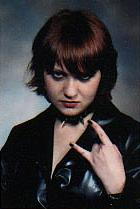
\includegraphics[width=1in,height=1.25in,clip,keepaspectratio]{figures/natalia.JPG}}]{Natalia Bilenko}
Natalia is a cool grad student with purple hair that studies brains.  She works in the Gallant lab in the Neuroscience department.
\end{IEEEbiography}

\begin{IEEEbiography}[{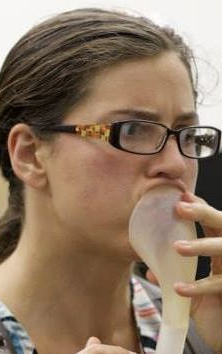
\includegraphics[width=1in,height=1.25in,clip,keepaspectratio]{figures/valkyrie.png}}]{Valkyrie Savage}
Valkyrie is a grad student whose desk is covered in 3D printed stuff.  She works for Bjoern Hartmann in the Berkeley Institute of Design.
\end{IEEEbiography}


% insert where needed to balance the two columns on the last page with
% biographies
%\newpage

% You can push biographies down or up by placing
% a \vfill before or after them. The appropriate
% use of \vfill depends on what kind of text is
% on the last page and whether or not the columns
% are being equalized.

%\vfill

% Can be used to pull up biographies so that the bottom of the last one
% is flush with the other column.
%\enlargethispage{-5in}



% that's all folks
\end{document}


